\section{Présentation des problématiques}\label{sec:intro:problematique}
Dans cette thèse, nous nous focalisons sur l'observations des données issues d'un système. Ainsi, nous considérons comme acquis la capacité à dialoguer d'une manière ou d'une autre avec le système observé pour récolter ses données comme présenté dans la figure~\ref{fig:intro:objectif:abstraction}. Dans cette section, nous présentons les problématiques soulevées par la gestion des données produites par ces systèmes.

\begin{figure}[ht]
\centering
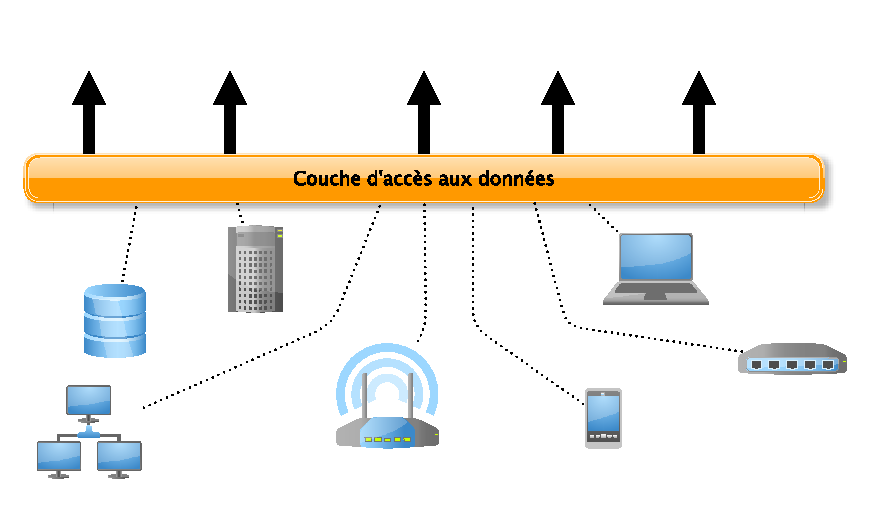
\includegraphics[width=0.7\textwidth]{intro-objectif}
\caption{Couche d'abstraction du système pour donner accès aux données}\label{fig:intro:objectif:abstraction}
\end{figure}

\subsection{Hétérogénéité des systèmes}
Plus l'informatique évolue, plus le nombre de dispositifs créés augmente. Grâce à l'émergence de l'informatique ubiquitaire, les dispositifs se font de plus en plus nombreux et de natures différentes. Ceci rend leur observation plus délicate car la surveillance des données d'un capteur est sensiblement différente à celle de l'utilisation d'un service d'hébergement web sur un serveur grande capacité.

Chaque système observé peut être représenté par \textbf{schéma de données} reposant sur un \textbf{modèle de données}. Ce schéma détermine la sémantique accordé au système. Ainsi, chaque système observé s'abstrait par un schéma différent et l'observation doit pouvoir s'adapter à chacun d'eux.

\subsection{Évolution des données du système}
Le système observé évolue au fur et à mesure du temps. Ce dynamisme introduit des problèmes majeurs d'un point de vue de la gestion des données. En effet, dans un système il existe deux grandes \textbf{catégories de données} : les données archivées et les données temps-réel. Les données archivées sont à évolution lente mais permet l'accès à des analyses de haut-niveau. Les données temps-réel sont des relevés instantanées et très volatiles indiquant l'état des entités du système (sous forme de flux de données).

Néanmoins, chacune de ces catégories possède des modèles de données et des traitements propres. Or, qu'elles soient temps-réel ou persistantes, ces données proviennent toutes du même système. Nous pouvons remarquer qu'il existe des ponts naturels entre ces deux catégories de données. En effet, les approches classiques de surveillance par l'archivage et l'analyse a posteriori montrent qu'un flux nécessite d'être considéré dans son ensemble pour être capable d'extraire de nouvelles connaissances. De la même manière, une donnée stockée peut subir des modifications déclenchant la production d'événements, ce qui est assimilable à un flux de données.

Ces processus de traitements de données sont assimilables à des interrogations que pose l'utilisateur sur l'ensemble des données. Il existe différent \textbf{modes d'interrogations} (ou requêtes). Ceux-ci reflètent l'hétérogénéité de l'évolution des données.
\begin{itemize}
    \item \textbf{Interrogation instantanée} : C'est la manière usuelle d'interroger dans les applications de gestion de base de données. L'utilisateur pose une question sur un ensemble de données considérées figées, du moins le temps du calcul de la réponse. Le système fournit une réponse représentative d'un état à un instant donné. Par exemple : \enquote{\it quel est l'ensemble actuel des équipements actifs de mon système}. La réponse à cette requête pourrait être \enquote{\it à cet instant, les équipements Box, PC1 et STB sont connectés et actifs}. La mention \enquote{\it à cet instant} est très importante, car si un nouvel équipement arrive dans le système, une nouvelle évaluation donnerait une réponse différente. Ainsi, cette interrogation correspond à la consultation ponctuelle de l'ensemble des données disponibles.
    \item \textbf{Interrogation continue} : C'est l'élément principal des systèmes événementiels, où les données sont considérés en constante évolution. L'utilisateur obtient ainsi une réponse qui évolue au cours du temps, sous forme de flux ou de mise à jour d'état. Un exemple pouvant être : \enquote{\it le flux de la charge moyenne du processeur sur une minute du PC1}. La réponse forme un flux continu d'information qui, toutes les minutes, reporte une nouvelle valeur moyenne pour ce capteur. Ainsi, la formation de processus de collecte ou de formation d'alerte suivent ce type d'interrogation.
\end{itemize}

Il est important de noter que ces deux paradigmes d'interrogation peuvent se combiner. Par exemple, il est possible d'effectuer un appel à une interrogation instantanée à l'intérieur d'un processus continu. De façon similaire, l'appel régulier d'une interrogation instantanée forme une réponse continue. Il est nécessaire que le système d'observation soit capable de manipuler naturellement ces deux types d'interrogation pour supporter le dynamisme des données.

\subsection{Hétérogénéité des données et traitement}
% On veut démontrer :
%       On subit les données fournies par le système et il faut les intégrer en un schéma commun
%       Pour intégrer et interroger les données, il nous faut de grandes capacités de traitement des données. via un langage qui a un pouvoir d'expression limité
La couche d'accès aux données permet d'exposer un ensemble de sources de données. Ces sources sont hétérogènes car chacune expose son propre schéma. De plus, certaines pourront fournir des données en temps-réel. Afin de pouvoir les interroger, il est nécessaire de les intégrer sur le schéma du système observé.

Afin de pouvoir intégrer et interroger les données, le système d'observation doit se doter de capacités de traitements des données. L'\textbf{expression} des traitements possibles se fait à travers d'un \textbf{langage}. Son paradigme sous-jacent définit la manière et la facilité d'adaptation à un système en particulier. Ce langage peut être dans le cas le plus extrême : un langage de programmation impératif bas niveau (comme le C par exemple). Dans ce cas, l'approche est très algorithmique, permettant une meilleure gestion des performances, mais une utilisation plus difficile et technique par la suite. À l'autre extrême, le langage peut être issu de la programmation logique permettant des performances moins contrôlées, mais une gestion globale déclarative, permettant une grande flexibilité.

Le langage utilisé peut avoir un \textbf{pouvoir d'expression} limité. Il est important d'être capable d'énumérer ce qui est possible d'exprimer. Les classes de logiques ou les équivalences à d'autres langages permettent de caractériser ces limitations. Par exemple, les opérations de manipulation de données pourrait être limitées par la logique du premier ordre, ou par le calcul relationnel.

\subsection{Adaptabilité à l'application}
Un des points critiques de la mise en œuvre d'un système d'observation est sa capacité à s'adapter à l'application finale. Plus la portée de l'observation est générique plus ce critère est important. Ainsi, il est important que le nombre et la complexité des procédures nécessaires à l'adaptation au système visé soit faible. Car, si un système est complet mais nécessite une adaptation longue et complexe, il devient difficile à mettre en pratique.

L'observation ne se justifie que par l'utilisation qui en est faite. En effet, pour tout système, il existe plusieurs \textbf{perspectives} possibles, car chaque utilisateur possède sa propre interprétation de l'observation. Cet angle de vue définit les données surveillées mais aussi la représentation du système observé. Il est nécessaire que le système d'observation s'adapte aux perspectives dans lesquelles se placent les utilisateurs.

Afin de pouvoir s'adapter aux besoins des utilisateurs, il est nécessaire que le système d'observation soit capable d'utiliser des \textbf{routines spécifiques} de traitement de données fournies par l'utilisateur. Cette extensibilité permet aussi bien l'intégration de tous types de besoins que l'amélioration des performances de traitements récurrents.

Enfin, pour que le système d'observation puisse être utilisable dans le plus grand nombre de contextes différents, il est nécessaire que les traitements de données soient performants. De plus, ce critère améliore la qualité des réponses en terme de latence de traitement. Le critère se mesure sur la capacité à traiter la charge d'un système en terme de nombre de sources ou en terme de débit supportés.

